% Part 2 opening chapter: from the virial partition (Chapter ch:virial_law, end of Part 1) to the cosmological coupling and its predictions.
% Source: the five Virial papers: Virial Efficiency (25 Feb 2026); Wide Domains (25 Feb 2026); Virial Partners (Mar 2026);
% Gravitational Decoherence and the Virial Partition (Mar 2026); The Thermodynamic Identity Governing the Virial Theorem (PRL version, 18 Mar 2026).
% Checks: docs/verification/virial/VIRIAL_CHECK.md, NBODY_TRACE.md.
% Read status: drafted 2026-10-02 after a read in which several chunks were previews only. All five re-read in full 2026-10-02 in 50-line chunks
% (ledger 277/641/674/560/222 lines, no gaps; book3/fullread/LEDGER_G3_Virial.md) and this chapter re-checked against them.

\chapter{The cosmological coupling $\beta_m=\Omega_m/2$}\label{ch:virial}

\section*{Overview}
IAM's Law (Chapter~\ref{ch:iams_law}) prices every classical record at $k_BT\ln2$ per bit on the nearest encoding surface. For matter
distributed through the universe the place is the cosmic horizon at the Gibbons--Hawking temperature. The law fixes the price; the virial
partition below fixes how much bound matter writes.
Part~\ref{part:1} closed with the virial partition: a stable $1/r$ system holds exactly half its binding energy as motion, and that half is the irreversible cost of the
binding transition (Chapter~\ref{ch:virial_law}). Applied to the universe, the same half fixes the coupling of the record term in the horizon first law,
$\beta_m=\Omega_m/2$, with no free parameter. This chapter derives the coupling and what follows from it --- the activation function, the growth coupling,
the amplitude of structure, the two expansion rates, and the tests that will decide it. Every later chapter in Part~\ref{part:2} uses this number.

\section{From the theorem to the cosmological coupling}
IAM adds to the horizon first law of Jacobson and Cai--Kim~\cite{Jacobson1995,CaiKim2005} the entropy of the classical records produced as matter decoheres gravitationally,
\begin{equation}
-dE=T_H\,d\!\left(S_{\rm geo}+S_{\rm info}\right).
\end{equation}
The share of the matter density that enters the record term is the kinetic half of the binding energy of collapsed structure. The virial theorem fixes it:
\begin{equation}
\beta_m=\frac{\Omega_m}{2}=0.15765\qquad(\Omega_m=0.3153,\ \text{Planck 2018}).
\end{equation}
The coupling is a prediction fixed by the measured matter density \derived; it enters every chain at this value and is never sampled.

It is useful to see where the $1/2$ sits in a real halo population. Writing $\beta_m=\Omega_m\,f_{\rm coll}\,\eta_{\rm vir}$, with $f_{\rm coll}$ the
fraction of matter in collapsed halos and $\eta_{\rm vir}$ the share of their binding energy in random, relaxed motion, the theorem requires
$f_{\rm coll}\eta_{\rm vir}=1/2$. Real halos are never perfectly relaxed: they are still accreting and merging (unrelaxed halos sit further from
equilibrium than relaxed ones), they carry ordered rotation, and some of their support is non-thermal (feedback, magnetic fields, cosmic rays). Each moves the
measured ratio away from the equilibrium value. In simulations, halos are conventionally called relaxed when $2T/|U|<1.35$ (Neto et al.\ 2007~\cite{Neto2007}), and the
mass-weighted population sits somewhat above 1. The decomposition is therefore a description of how the equilibrium value is approached in a population,
not a separate confirmation of it; $\beta_m=\Omega_m/2$ rests on the theorem.
Simulations measure the equilibrium directly: within the virial radius halos have $2T/|U|\approx1.1$--$1.3$ (Bett et al.\ 2007~\cite{Bett2007}; Neto et al.\ 2007~\cite{Neto2007};
Power et al.\ 2012~\cite{Power2012}), and $1.02$--$1.17$ once the pressure of still-infalling matter at the boundary is included (Klypin et al.\ 2016~\cite{Klypin2016}). The theorem holds in
the halo population to within the infall still under way (Chapter~\ref{ch:virial_law}).

\section{What the coupling predicts}
\subsection{The activation function and the growth coupling}
The record accumulates as structure forms. Integrating the record rate through the horizon first law gives the activation function
\begin{equation}
E(a)=\exp\!\left(1-\frac1a\right)=e^{-z},
\end{equation}
with $E\to0$ at early times ($E(z{=}10)=4.5\times10^{-5}$), $E(1)=1$ today, $dE/da>0$ throughout, and $E\to e$ as $a\to\infty$. It reaches 10, 50 and
90\,\% of today's value at $z=2.30$, $0.69$ and $0.11$. Matter perturbations grow with the effective coupling
\begin{equation}
\ddot\delta_m+2H\dot\delta_m-\tfrac32\Omega_mH_0^2a^{-3}\mu(a)\,\delta_m=0,\qquad
\mu(a)=\frac{H^2_{\Lambda{\rm CDM}}(a)}{H^2_{\Lambda{\rm CDM}}(a)+\beta_mE(a)H_0^2},\label{part2:eq:mu_virial}
\end{equation}
while light is unaffected, $\Sigma=1$: photons on null worldlines accumulate no proper time and take no part in decoherence. This is the
$\mu$--$\Sigma$ form used in the Level~1 chains. The Level~2 chains put the same term into the friction on matter perturbations instead
(Chapter~\ref{ch:level2}); the two give the same growth to within a few tenths of a percent.

The rate at which the record is written, $dE/d\ln a=E/a$, peaks exactly at $a=1$; $E$ itself has its inflection at $a=1/2$.

\paragraph{The exponent.} The record-writing rate is $\dot I\propto\rho_mD^nfH$, accumulated on the horizon as $dS_{\rm info}/dt=\dot I/(T_HA_H)$
(Chapter~\ref{ch:iams_law}). In matter domination this gives $S_{\rm info}\propto a^{\,n-9/2}$; the $-1/a$ in $E(a)$ requires $n-\tfrac92=-1$, so $n=\tfrac72$.
The full $\Lambda$CDM integration finds the closest fit for $D^{7/2}$. $E(a)$ itself does not depend on $n$.

\begin{center}\small
\begin{tabular}{cccc}
\hline
$z$ & $E(a)$ & $\mu$ & coupling reduced by ($1-\mu$)\\\hline
0 & 1.000 & 0.864 & 13.6\,\%\\
0.3 & 0.741 & 0.922 & 7.8\,\%\\
0.5 & 0.607 & 0.948 & 5.2\,\%\\
0.7 & 0.497 & 0.966 & 3.4\,\%\\
1.0 & 0.368 & 0.982 & 1.8\,\%\\\hline
\end{tabular}
\end{center}
Values from Eq.~\eqref{part2:eq:mu_virial} \calc.

\subsection{Amplitude of structure}
In the Planck chains $\sigma_8$ moves from $0.809$ to $0.800$ (Level 2; from $0.814$ to $0.802$ at Level 1) \measured, while $H_0$, $\Omega_bh^2$ and $\Omega_m$ stay within $0.1\sigma$
of their $\Lambda$CDM values (Level~2): the lower amplitude is growth physics, not a parameter shift. The Level 2 chain gives $S_8=0.822\pm0.011$, in line with the
KiDS-Legacy cosmic-shear value $S_8=0.815^{+0.016}_{-0.021}$~\cite{Wright2025}.

\subsection{Two expansion rates}
Photon-sector probes (CMB acoustic scale, BAO angles) read the $\Lambda$CDM rate; matter-sector probes calibrated on timelike worldlines read
\begin{equation}
H_0^{(m)}=H_0^{(\gamma)}\sqrt{1+\beta_m}=67.16\times1.0759=72.26\ \text{km\,s}^{-1}\text{Mpc}^{-1}
\end{equation}
(Level 2 chain; with Planck's $67.36$, $72.48$) \derived. SH0ES measures $73.04\pm1.04$~\cite{Riess2022} ($0.75\sigma$); Planck $67.36\pm0.54$~\cite{Planck2018VI} against the chain's $67.16\pm0.47$
($0.37\sigma$). Supernova distances follow $\Lambda$CDM geometry; their $H_0\approx73$ comes from the Cepheid calibration (Chapter~\ref{ch:dsvalidation}).

\subsection{Growth and geometry give different $\Omega_m$}

\begin{figure}[htbp]\centering
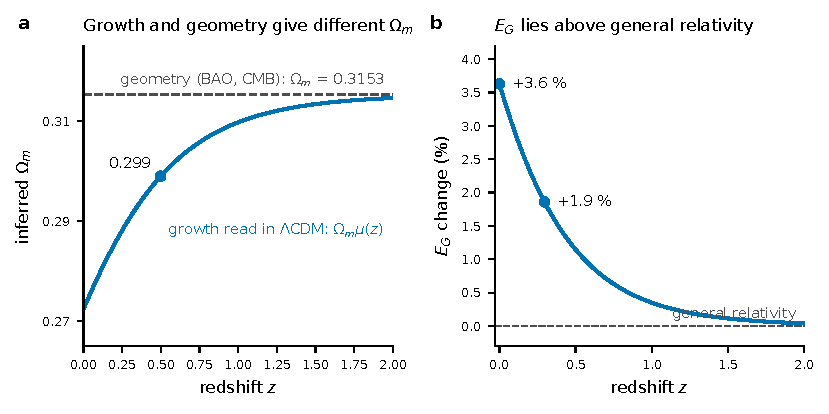
\includegraphics[width=\textwidth]{figures/part2/fig_growth_vs_geometry.pdf}
\caption{(a) The matter density a growth-only measurement infers in $\Lambda$CDM, $\Omega_m\mu(z)$ (0.299 at $z=0.5$), against the geometric $\Omega_m=0.3153$ that distances keep. (b) The change in $E_G$ with $\Sigma=1$, $f_{\Lambda\rm CDM}/f_{\rm IAM}-1$ from the linear growth equation with the same early amplitude: $+3.6\,\%$ today and $+1.9\,\%$ at the BGS redshift $z=0.295$. \prediction}\label{fig:growth_vs_geometry}
\end{figure}
A growth-only measurement interpreted in $\Lambda$CDM infers $\Omega_m^{\rm growth}(z)=\Omega_m\,\mu(z)$: $0.299$ at $z=0.5$, $5.2\,\%$ below the
geometric value \calc, while distances (BAO, the CMB acoustic scale) keep the geometric $\Omega_m$. Combined full-shape plus BAO values, such as DESI DR1's
$\Omega_m=0.2962\pm0.0095$~\cite{DESI2024VII}, are dominated by the distance information and are not a growth-only measurement. The clean test fits the full-shape growth
with a template built from the modified growth and compares it with the BAO geometry of the same survey.

\subsection{The $E_G$ statistic}
$E_G$ compares galaxy--lensing cross-correlation with galaxy clustering and velocities~\cite{Zhang2007EG}. With $\Sigma=1$ the lensing kernel is unchanged and the growth rate is
lower, so $E_G=\Omega_m/f_{\rm IAM}(z)$ lies above the general-relativity value at every redshift. All the input data are published; the comparison with the
IAM growth curve is a direct near-term test.

\subsection{The virial ratio through cosmic history}

\begin{figure}[htbp]\centering
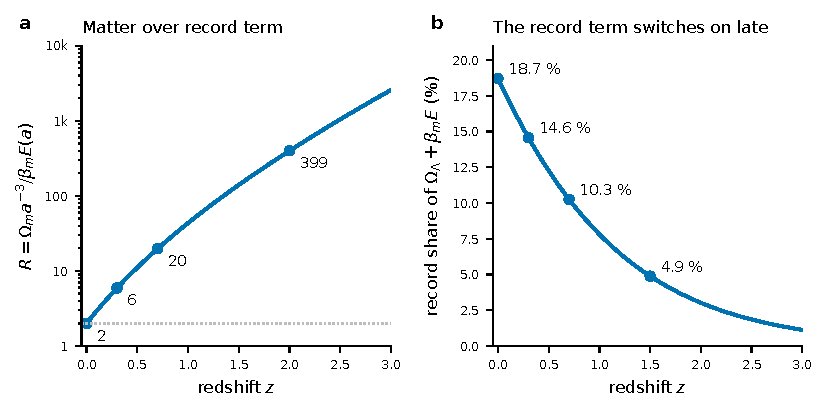
\includegraphics[width=\textwidth]{figures/part2/fig_record_history.pdf}
\caption{(a) Matter over the record term, $R(a)=\Omega_ma^{-3}/\beta_mE(a)$: 399 at $z=2$, 20 at $z=0.7$, 6 at $z=0.3$ and 2 today, the last by construction. (b) The record term's share of $\Omega_\Lambda+\beta_mE(a)$ in the matter-sector rate: 18.7, 14.6, 10.3 and 4.9\,\% at $z=0$, 0.3, 0.7 and 1.5. Planck 2018 background, $\Omega_m=0.3153$, $\beta_m=0.15765$. \calc}\label{fig:record_history}
\end{figure}
The ratio of the matter density to the record term, $R(a)=\Omega_ma^{-3}/[\beta_mE(a)]$, is $399$ at $z=2$, $20$ at $z=0.7$, $6$ at $z=0.3$, and $2$
today --- the last by construction, since $\beta_m=\Omega_m/2$ and $E(1)=1$. In the matter-sector rate $H_m^2$, matter equals the vacuum plus record term at $z=0.361$ ($\Lambda$CDM:
$0.295$). Today the record term is $18.7\,\%$ of $\Omega_\Lambda+\beta_m$; at $z=0.3$, $0.7$ and $1.5$ it is $14.6$, $10.3$ and $4.9\,\%$. The reading of
$R=2$ as the solution of the coincidence problem is interpretation and is taken up in Part~\ref{part:5} (Chapter~\ref{ch:theoryinterp}).

\section{Tests}
\begin{itemize}
\item \emph{Euclid} measures growth (spectroscopy) and lensing (imaging) on the same volume~\cite{Euclid2025}. The prediction is $\mu_0=\mu(0)-1=-0.136$ with $\Sigma_0=0$ \prediction.
Euclid's published forecasts bracket the test of the IAM $\mu(z)$ from about $0.3\sigma$ (conservative scale cuts) to about $7\sigma$ (smallest
scales modelled), and a forecast made with the IAM $\mu(z)$ itself is still to be done (Chapter~\ref{ch:latetime}). The clustering and weak-lensing products of DR1 are expected in mid-2027~\cite{ESA2026DR1}.
\item \emph{DESI Year 5}: $f\sigma_8$ is forecast to about $1\,\%$ per $\Delta z=0.1$ bin at $0.8<z<1.3$ and $0.4$--$0.7\,\%$ aggregated over all redshifts~\cite{DESI2016}.
The predicted suppression grows toward the present as $E(a)$ activates ($4.25\,\%$ at $z=0$, $2.17\,\%$ at $z=0.3$, $1.35\,\%$ at $z=0.5$, $0.41\,\%$ at $z=1$;
linear growth, Planck 2018 background, same early amplitude) \prediction, not a constant rescaling.
\item $E_G$ from published galaxy--lensing data.
\item What would count against the virial coupling: $\mu_0$ consistent with zero at a precision that excludes $-0.136$; correlated $\mu\neq1$, $\Sigma\neq1$; a
redshift-independent growth suppression; or, with $\Omega_m$ revised, growth data that still require the old $\beta_m$.
\end{itemize}

The reading of dark matter and dark energy as the two halves of the virial partition, the coincidence and the arrow of time are interpretation; they are
taken up in Part~\ref{part:5} (Chapters~\ref{ch:theoryinterp} and~\ref{ch:synthesis}). Whether the DESI preference for evolving dark energy is an artefact of
fitting one fluid to two sectors is open until the two-ruler test is run on real data (Chapter~\ref{ch:sectortension}) \openprob.
